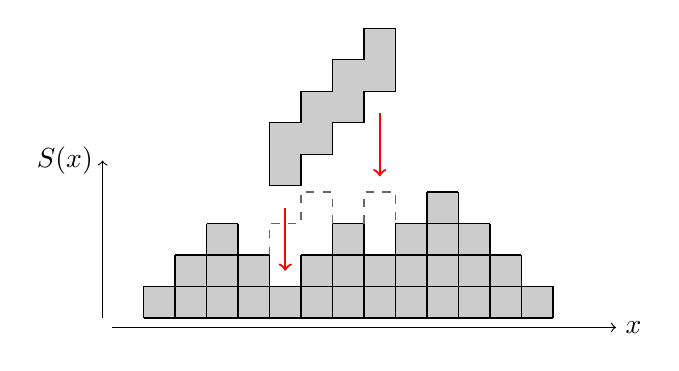
\begin{tikzpicture}[scale = .4]
\draw[->] (0, -.3) -- (16,-.3) node[right]{$x$};
\draw[->] (-.3,0) -- (-.3,5) node[left]{$S(x)$};
\fill[black!20] (1,0) -- (1,1) -- (2,1) -- (2,2) -- (3,2) -- (3,3) -- 
     			(4,3) -- (4,2) -- (5,2) -- (5,1) -- (6,1) -- (6,2) -- (7,2) -- (7,3) -- (8,3) -- (8,2) -- (9,2) -- (9,3) -- (10,3) -- (10,4) 
     			 -- (11,4) -- (11,3) -- (12,3) -- (12,2) -- (13,2) -- (13,1)  -- (14,1) -- (14,0);
     			 
\draw (1,0) -- (14,0);
\draw (1,1) -- (14,1);
\draw (2,2) -- (5,2);
\draw (6,2) -- (13,2);
\draw (3,3) -- (4,3);
\draw (7,3) -- (8,3);
\draw (9,3) -- (12,3);
\draw (10,4) -- (11,4);
\draw (1,0) -- (1,1);
\draw (2,0) -- (2,2);
\draw (3,0) -- (3,3);
\draw (4,0) -- (4,3);
\draw (5,0) -- (5,2);
\draw (6,0) -- (6,2);
\draw (7,0) -- (7,3);
\draw (8,0) -- (8,3);
\draw (9,0) -- (9,3);
\draw (10,0) -- (10,4);
\draw (11,0) -- (11,4);
\draw (12,0) -- (12,3);
\draw (13,0) -- (13,2);
\draw (14,0) -- (14,1);

\draw[fill=black!20] (5,5.2) -- (5,4.2) -- (6,4.2) -- (6,5.2) -- (7,5.2) --  
                     (7,6.2) --
					 (8,6.2) -- (8,7.2) -- (9,7.2) -- (9,8.2) -- (9,9.2) -- (8,9.2)
					 -- (8,8.2) -- (7,8.2) -- (7,7.2) -- (6,7.2) -- (6,6.2) -- (5,6.2)
					 -- (5,5.2);
\draw[thick, ->, red] (5.5,3.5) -- (5.5,1.5);
\draw[thick, ->, red] (8.5,6.5) -- (8.5,4.5);

\draw[dashed, black!60] (5,2) -- (5,3) -- (6,3) -- (6,4) -- (7,4) -- (7,3);
\draw[dashed, black!60] (8,3) -- (8,4) -- (9,4) -- (9,3);
\end{tikzpicture}
%\begin{tikzpicture}[scale = .3, cross/.style={path picture={ 
%		\draw[black]
%		(path picture bounding box.south east) -- (path picture bounding box.north west) (path picture bounding box.south west) -- (path picture bounding box.north east);
%}}]
%
%\draw[->] (0, -.3) -- (16,-.3) node[right]{$x$};
%\draw[->] (-.3,0) -- (-.3,5) node[left]{$S(x)$};
%\fill[black!20] (0,0) -- (3,3) -- (5,1) -- (7,3) -- (8,2) --
%(10,4) -- (14,0) ;
%\draw (0,0) -- (3,3);
%\draw (2,0) -- (4,2);
%\draw (4,0) -- (7,3);
%\draw (6,0) -- (10,4);
%\draw (8,0) -- (11,3);
%\draw (10,0) -- (12,2);
%\draw (12,0) -- (13,1);
%\draw (2,0) -- (1,1);
%\draw (4,0) -- (2,2);
%\draw (6,0) -- (3,3);
%\draw (8,0) -- (6,2);
%\draw (10,0) -- (7,3);
%\draw (12,0) -- (9,3);
%\draw (14,0) -- (10,4);
%\draw[dashed, black!60]  (5,3) -- (6,4);
%\draw[dashed, black!60]  (7,3) -- (6,4);
%\draw[dashed, black!60]  (6,2) -- (5,3);
%
%\draw[fill=black!20] (5,6) -- (6,5) -- (7,6) -- (6,7) -- (5,6);
%\draw[thick, ->, red] (6,4.5) -- (6,3);
%%\node [draw,circle,cross,minimum width=1](B) at (6,3.5){}; 
%\end{tikzpicture}
